\documentclass{zettel}

%\renewcommand{\gregor}{\put(10.0,-3.5){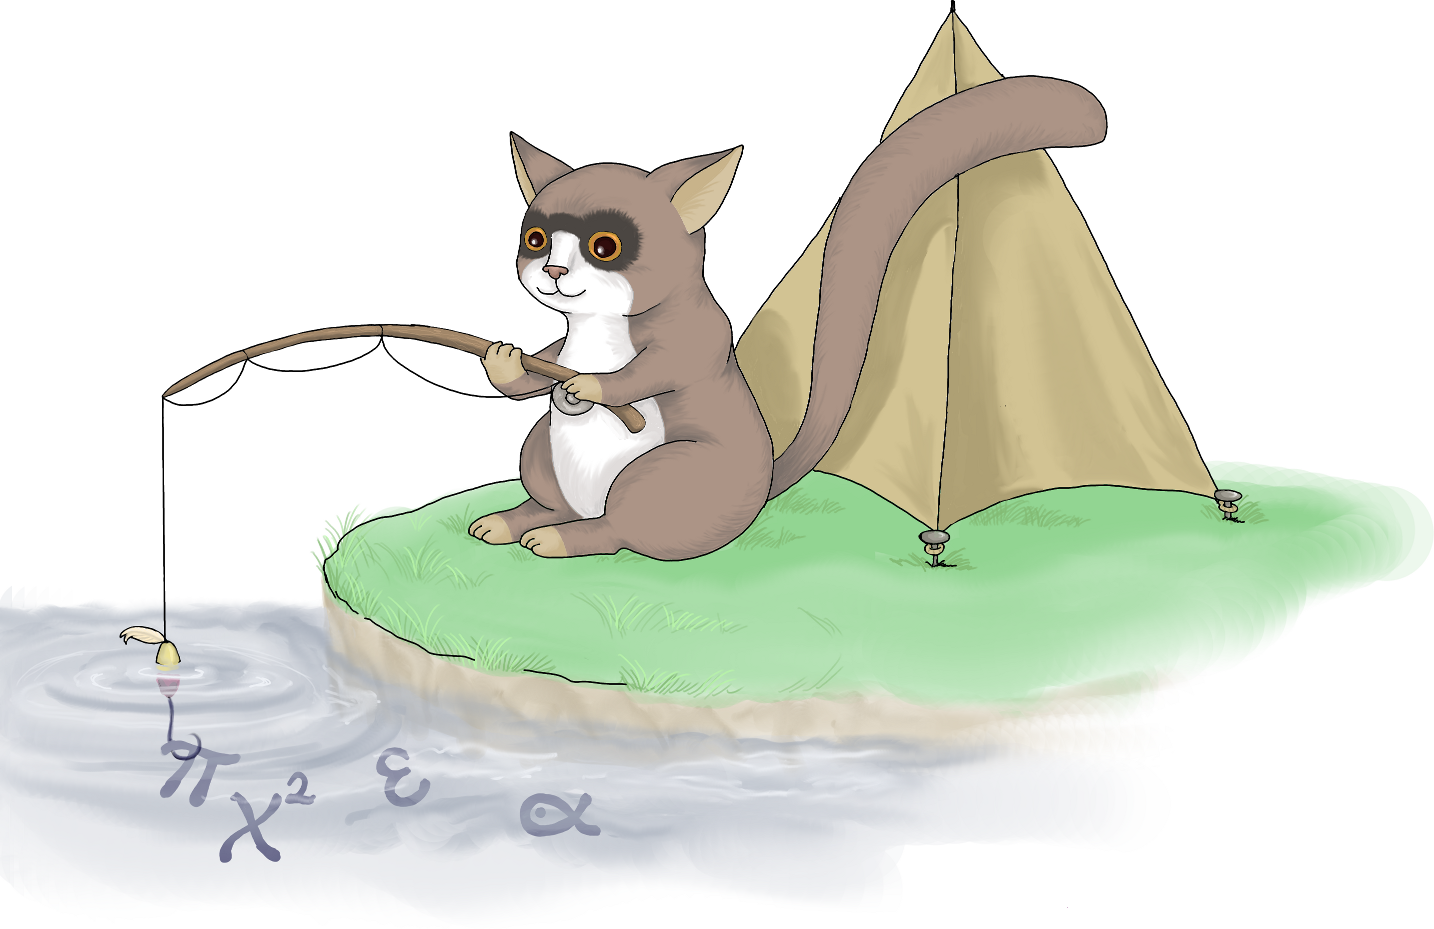
\includegraphics[scale=0.18]{campgregor}}}

\usepackage{framed}
\definecolor{shadecolor}{rgb}{.97,.97,.97}

\geometry{tmargin=1.5cm,bmargin=1.5cm,lmargin=2.5cm,rmargin=2.5cm}

\renewcommand{\gregor}{\put(13.2,-3.0){
\includegraphics[scale=0.18]{cover}}}
\begin{document}

\renewcommand{\betreff}{Mathecamp des Matheschülerzirkels Augsburg vom 16. bis
20. August}

\makeletterhead{}
\begin{picture}(0,0)
  \put(8.7,-19){%
    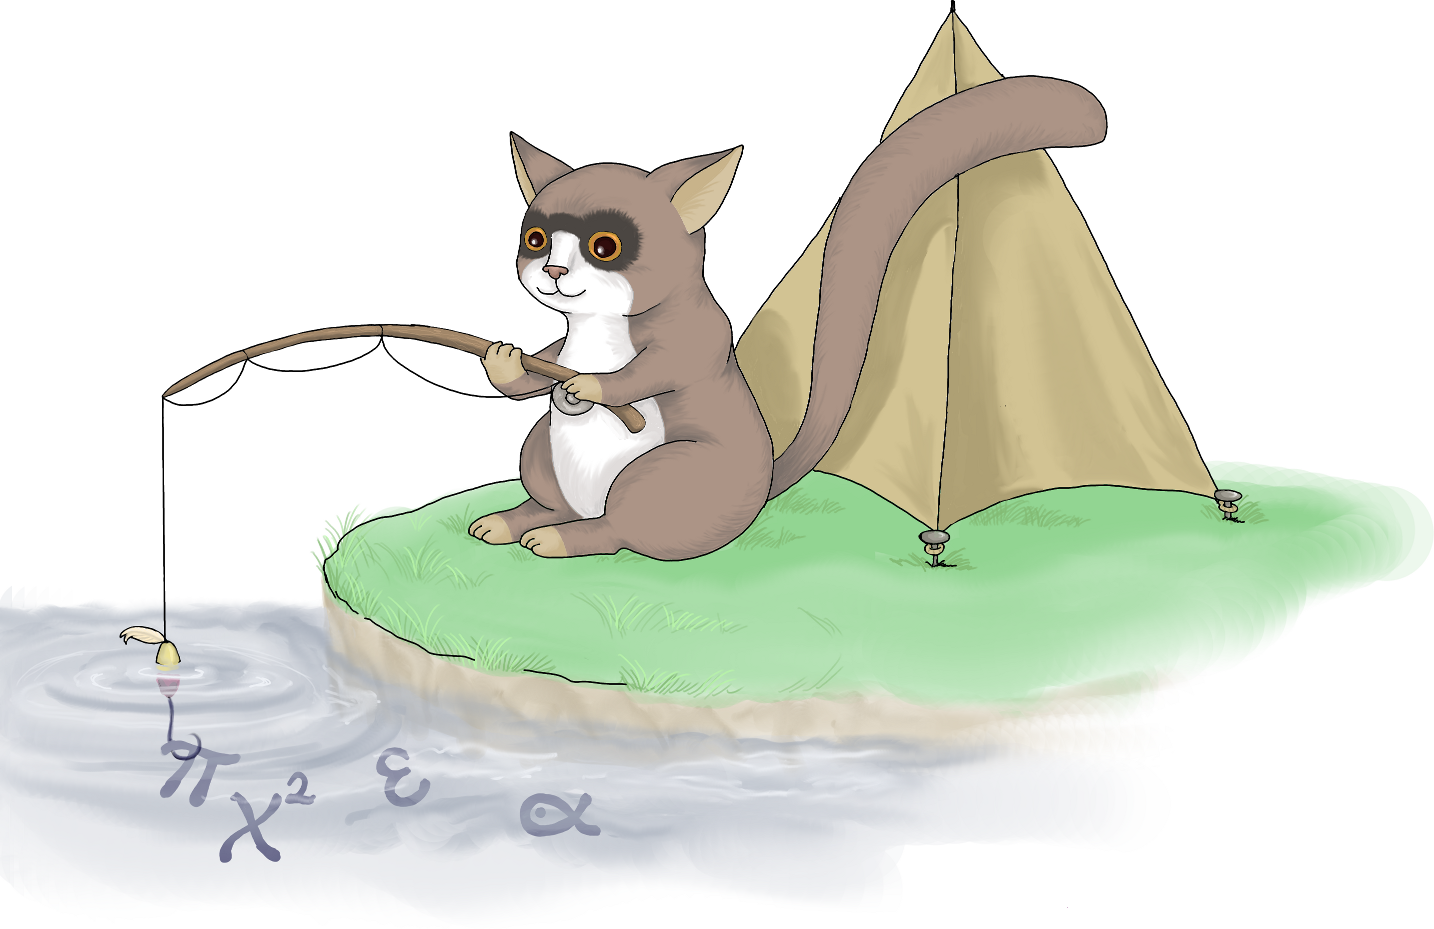
\includegraphics[scale=0.18]{campgregor}
  }
\end{picture}
\vspace{-2em}

Liebe Schülerinnen und Schüler, liebe Eltern,

wir laden euch herzlich zum ersten Mathecamp des Matheschülerzirkels Augsburg
ein. Dort werden wir mit euch tolleXXXspannende mathematische Themen verstehen und die
Freizeit in den Ferien genießen. XXX Gleichgesinnte

\begin{tabbing}
  \hspace{2.2cm} \= \kill
  \textbf{Was?} \> Mathematik und Spaß in den Ferien \\[0.3em]
  \textbf{Wann?} \> 16. bis 20. August 2014 (Samstag bis Mittwoch) \\[0.3em]
  \textbf{Wo?} \> Bruder-Klaus-Heim in Violau, Schullandheim der Diözese
  Augsburg \\[0.3em]
  \textbf{Für wen?} \> \begin{minipage}[t]{\dimexpr\textwidth-2.3cm}
  Einzige Teilnahmevoraussetzung ist Spaß und Interesse an
  Mathematik.
  Jeder kann mitkommen, auch, wenn man nicht bei den Zirkeln
  mitgemacht hat.\end{minipage} \\[0.3em]
  \textbf{Kosten?} \> 60,-- \texteuro
\end{tabbing}

An jedem Tag werden zwei Arbeitsgruppen stattfinden. Dabei behandeln wir spannende
Bereiche der Mathematik, die wir in den Präsenz- und Korrespondenzzirkeln noch nicht gesehen haben.
Selbstverständlich gibt es für verschiedene Altersstufen angepasste Kurse
mit verschiedenen Themen und Schwierigkeiten statt, sodass immer für jeden
etwas dabei ist.

Daneben stehen Spiele- und Bastelstunden sowie die Nutzung der
Sternwarte des Heims auf dem Programm. Natürlich hoffen wir auf
schönes Wetter, damit wir auch die Tiere auf dem Gelände besuchen
und am Abend am Lagerfeuer grillen und Musik machen können.
Weiterhin stehen uns eine Pizzabäckerei, ein Volleyballplatz und ein
Fußballplatz zur Verfügung, sodass es sicher niemandem langweilig
wird. Außerdem wird es zwei Vorträge von
einer auswärtigen Mathematikerin und einem Mathematiker geben.

Getragen wird das Camp vom Mathematisch-Physikalischen Verein e.\,V.
Das Betreuer- und Organisationsteam um Sven Prüfer und Kathrin Helmsauer
besteht aus Doktoranden und Mitarbeitern des Instituts, die in
ihrer Freizeit ehrenamtlich interessierten Schülern Mathematik näherbringen wollen.
Sowohl Sven als auch mehrere weitere Betreuer haben bereits Erfahrungen in der
Jugendarbeit und beim Betreuen von Ferienlagern.

Wenn ihr teilnehmen möchtet, bittet eure Eltern das beiliegende Anmeldeformular
bis zum 12. Juli 2014 auszufüllen und an uns zurückzuschicken.
\vspace{\medskipamount}

\begin{minipage}{0.54\textwidth}
Dank finanzieller Unterstützung durch das Institut für Mathematik konnten wir
den Eigenbeitrag von circa 200~\texteuro{} deutlich reduzieren, er beläuft sich
jetzt auf 60~\texteuro. In diesem Betrag sind die Kosten für An- und Abreise,
Unterkunft, Verpflegung und Freizeitaktivitäten enthalten. Wir Betreuer
arbeiten ehrenamtlich. XXX muss noch in die neuen Formulierungen eingearbeitet
werden.
\end{minipage}

\newpage

Der niedrige Teilnahmebeitrag ist nur durch eine großzügige und
einmalige finanzielle Unterstützung des Instituts für Mathematik
möglich, das die restlichen 130~\texteuro{} pro Teilnehmer übernimmt.
Falls Sie unsere Arbeit unterstützen und dadurch auch
zukünftig Veranstaltungen dieser Art ermöglichen möchten, können
Sie gerne einen höheren Betrag überwiesen. Als gemeinnütziger
Verein stellen wir dann eine Spendenbescheinigung über den
zusätzlichen Betrag aus.

Wir bitten, den Betrag bis zum 1. August 2014 auf unser Konto zu überweisen.
Familien, die sich den
Eigenbeitrag nicht leisten können, bitten wir, mit uns Kontakt aufzunehmen. Im
Rahmen der finanziellen Möglichkeiten des Vereins können wir gegebenenfalls
auf den Beitrag verzichten.

\vspace{-0.7em}
\begin{tabbing}
  \qquad\qquad \= Verwendungszweck:\, \= \kill
  \> Kontoinhaber: \> Matheschülerzirkel Augsburg \\
  \> Konto-Nr.: \> 12345678 \\
  \> BLZ: \> 12345678 \\
  \> IBAN: \> 2437243784237878342 \\
  \> BIC: \> 23487432789432 \\
  \> Betrag: \> 70,-- \texteuro (XXX Bettwäsche) \\
  \> Verwendungszweck: \> Mathecamp \emph{Vorname Nachname}
\end{tabbing}
\vspace{-0.7em}

Das Camp beginnt am 16. August zwischen 10:00 Uhr und 11:00 Uhr. Ihr könnt
entweder individuell zu dieser Zeit anreisen oder euch um 09:30 Uhr auf dem Campus der
Universität einfinden, um dann gemeinsam mit uns im Reisebus nach Violau zu fahren.

Die Abreise ist am 20. August ab 16:30 Uhr. Ihr könnt euch entweder von euren
Eltern abholen lassen oder mit uns zurück nach Augsburg fahren. Dort kommen wir
gegen 17:30 Uhr an der Universität an.

Wir schicken euch Ende Juli eine Übersicht mit
letzten Details und Kontaktdaten vor Ort. Bei Fragen stehen wir euch jederzeit
zur Verfügung. Bitte zögert nicht, uns dazu telefonisch unter 0821/598-5805 oder per
Mail an \textsf{mathezirkel@math.uni-augsburg.de} zu kontaktieren.

Wir hoffen, dass ihr euch auf das Mathecamp genauso freut wie wir und dass wir
euch dort begrüßen dürfen!

\vspace{2em}

Euer Team vom Mathecamp

Kathrin Helmsauer \\
Sven Prüfer \\
weitere Namen, alphabetisch (um Vertrauen in uns zu stärken)

\vfill

XXX: Laut einer Website gibt es im Bruder-Klaus-Heim auch:
Fußballplatz, Volleyballplatz, Spielgeräten, Wasserspielen, Indianerzelten,
Lagerfeuerstelle, Grillplätzen, Pizzaofen, Strohstadel, Zeltplatz, Tieren
(Pferde, Ponys, Schafe, Ziegen, Lamas, Hasen, Meerschweinchen, Enten), See
(Boot fahren). Können wir auf eine gute Art und Weise die Tiere erwähnen?

%Übrigens organisieren wir vom 16. bis 20. August ein Mathecamp in Violau. Dort
%bieten wir euch spannende mathematische Kurse und Workshops, etwa zu geheimen
%Botschaften, Fraktalen, Knobelaufgaben, Geometrie, Nim-Spielen oder anderen
%Themen. Daneben gibt es bei unserer Unterkunft auch verschiedene Möglichkeiten
%zur Freizeitgestaltung, unter anderem ein Teleskop, eine Pizzabäckerei und
%Outdoor-Aktivitäten. Wir sind gerade auf Sponsorensuche und werden euch in
%einem Monat nähere Informationen schicken. Wenn ihr Interesse habt, sagt euren
%Eltern schon mal den Termin!

\end{document}

XXX: Euro-Zeichen
